\chapter{Definizione del problema}
\setcounter{section}{1}
Nell'ambiente \textit{Cloud} l'archiviazione corretta e lo scambio di dati \`{e} di vitale importanza. L'obiettivo \`{e} quello di ottenere una amministrazione professionale dello \textit{storage}.\\
\`{E} necessario quindi esaminare la gestione e la manutenzione di un insieme di copie di dati, in modo che sia il pi\`{u} efficiente possibile, al fine di tutelare il dato in qualsiasi caso di perdita o di danneggiamento ai dischi.\\

La replicazione dati \`{e} un trasferimento dati unidirezionale da uno o pi\`{u} nodi che permette:
\begin{itemize}
\item 
l'aumento di affidabilit\`{a} del sistema, rendendo il sistema tollerante ai guasti;
\item
miglioramento delle prestazioni del sistema, aumentandone la scalabilit\`{a}.
\end{itemize}

Tuttavia la replicazione pu\`{o} causare la presenza di eccessive copie di un dato, causando perfino problemi di consistenza. La potenziale modifica di un dato replicato implica che le sue rispettive repliche siano aggiornate. \\
Per questo \`{e} necessario trovare un adeguato compromesso del numero di repliche, pur mantenendo garanzia, sicurezza e buone performance.\\

Mantenere la disponibilit\`{a} del servizio realizzato, sostenere correttamente eventuali guasti dei server, rispettare la giusta partizione della rete e gestione delle disconnessioni sono le principali finalit\`{a} da raggiungere.\\
La tolleranza ai guasti garantisce dati corretti e aggiornati in caso di un eventuale guasto. Per un numero \verb"N" di guasti occorre avere un numero sufficiente di copie del dato e del metadato, consentendo in questo modo di ottenere nuovamente l'oggetto perso.\\

In questa tesi viene analizzato qual \`{e} il modo pi\`{u} proficuo per eseguire la replicazione di un file in \textit{upload}, allo scopo di distruibuire i dati uniformemente.\\ Oltre a ci\`{o}, sono esaminati alcuni lanci di configurazione che hanno portato a una specifica scelta architetturale che garantisca la ridondanza di un dato, mantenendo buone performance.

Un file \`{e} suddiviso in \textit{chunk} di varie dimensioni e, rispetto ai metadati, occupano gran parte del disco. I metadati rappresentano l'informazione anagrafica del dato e hanno dimensione fissa.

La replicazione dei metadati, \`{e} essenzialmente gestito da Pglogical, implementato come estensione di PostgreSQL. \\
\`{E} un sistema logico di replica, alternativo alla replica fisica, poich\`{e} consente di replicare i metadati in modo altamente pi\`{u} efficiente. Segue il modello di \textit{publish/subscriber} e permette l'utilizzo della replica selettiva di database.

Per la copia dei dati la metodologia adoperata \`{e} pi\`{u} semplice: sar\`{a} sufficiente lanciare una query in parallelo che permette la scrittura dei \textit{chunk} su due differenti dischi.

Grazie a queste configurazioni \`{e} possibile ottenere almeno una doppia ridondanza del dato in modo sicuro e corretto, mantenendo il sistema affidabile.

\item
\subsection{Cluster di database}
Un cluster \`{e} una raccolta di componenti che garantisce scalabit\`{a} e disponibilit\`{a} distribuendone i costi. Un cluster di database (SQL usa il termine cluster di catalogo) \`{e} una collezione di database gestiti da una singola istanza di un server database in esecuzione. Un'istanza \`{e} la raccolta di memoria e processi che interagiscono con un database, cio\`{e} l'insieme di file fisici che effettivamente memorizzano i dati\cite{etichetta1}. A tal fine, \`{e} possibile creare un cluster di database per applicazioni \textit{enterprise high-end}, memorizzando e elaborando informazioni sui nodi.\\ L'architettura per un cluster di database \`{e} distinta da come le responsabilit\`{a} dei dati sono condivise tra i nodi di calcolo.

Seguono due dei vantaggi principarli offerti dal clustering, specialmente in un ambiente di database di alto volume:
\begin{itemize}
\item 
\textit{Fault tolerance} (tolleranza ai guasti): in caso di guasto del singolo server, il cluster offre un'alternativa, in quanto esiste pi\`{u} di un server o istanza per gli utenti a cui connettersi;
\item
\textit{Load balancing} (bilanciamento del carico): la funzionalit\`{a} di clustering \`{e} generalmente impostata per consentire agli utenti di essere assegnati automaticamente al server con il minor carico\cite{etichetta1}. 
\end{itemize}
Ci sono differenti tipi di architetture clustering che si diversificano da come vengono memorizzati i dati e allocate le risorse.\\
La prima modalit\`{a} di clustering \`{e} conosciuta come architettura "\textit{shared-nothing}" (SN). \`{E} un'architettura di elaborazione distribuita in cui ogni nodo/server \`{e} totalmente indipendente e autonomo, pertanto nessuno dei nodi condivide memoria o archiviazione del disco. Pi\`{u} generalmente, non esiste un unico punto di contesa nel sistema\cite{etichetta5}. Il partizionamento \`{e} tale che ogni nodo possiede un sottoinsieme dei dati, ovvero ogni nodo ha accesso esclusivo su quel particolare sottoinsieme\cite{etichetta2}.\\

\begin{figure}[htbp]
\centering
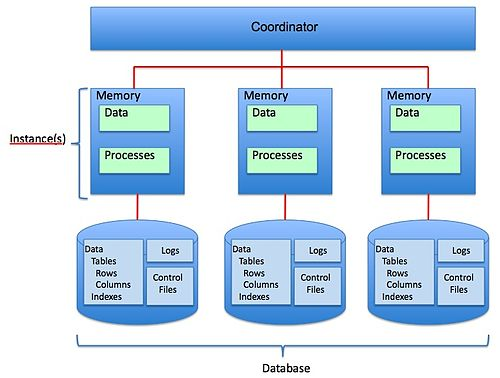
\includegraphics[scale=0.70]{img/Shared_Nothing_Architecture.jpg}\\
\caption{Architettura \textit{shared-nothing}\cite{etichetta5}.}
\label{fig:Shared_Nothing_Architecture}
\end{figure}

I vantaggi dell'architettura SN rispetto a un'entit\`{a} centrale che controlla la rete (un'architettura basata su controller) riguarda l'eliminazione di qualsiasi singolo punto di guasto, consentendo funzionalit\`{a} di auto-riparazione (\textit{self-healing}) e fornendo un vantaggio nell'offrire aggiornamenti non distruttivi\cite{etichetta6}. 
%\textbf{DA LEGGERE PER BENE ARTICOLO CITATO.}
\textit{Shared-nothing} \`{e} anche noto come "\textit{database sharding}". \\
In generale, un sistema SN divide i suoi dati in vari nodi su database diversi o pu\`{o} richiedere a ciascun nodo di mantenere la propria copia dei dati dell'applicazione utilizzando un qualche tipo di protocollo di coordinamento\cite{etichetta5}.\\


Si oppone a quest'ultima, l'architettura nota come "\textit{shared-disk}" (disco condiviso), in cui tutti i dati vengono memorizzati centralmente in un unico disco e sono accessibili da tutti i nodi di cluster\cite{etichetta7}.\\
In questo tipo di struttura pi\`{u} istanze di database vengono raggruppate in un singolo database sul disco. Nei sistemi di dischi condivisi, i blocchi (o pagine) di dati su disco possono avere un solo proprietario.
%La propriet\`{a} dei blocchi (o pagine) viene trasferita all'istanza che sta facendo l'aggiornamento. Questo genera traffico di rete e in genere un'infrastruttura dedicata viene implementata tra le istanze di database per far fronte a questo traffico.))
L'architettura \textit{shared-disk} \`{e} un esempio di \textit{Synchronous multi-master}, ovvero ogni istanza del database pu\`{o} scrivere (cio\`{e} \`{e} un master) in modo sincrono\cite{etichetta7}.

\begin{figure}[htbp]
\centering
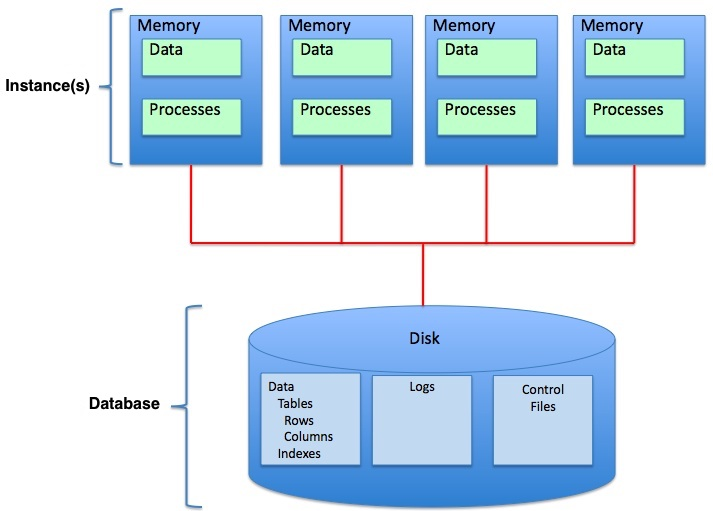
\includegraphics[scale=0.50]{img/Shared_Disk_Architecture.jpg}\\
\caption{Architettura \textit{shared-disk} \cite{etichetta7}.}
\label{fig:Shared_Disk_Architecture}
\end{figure}
\\

In un'architettura SD, grandi reti di computer possono operare su un singolo set di dati senza la necessit\`{a} di replicare o bloccare quel set di dati\cite{etichetta7}.
\textit{Shared disk} ha due vantaggi:
\begin{itemize}
\item
ogni processore ha la propria memoria; 
\item
il bus di memoria non \`{e} un collo di bottiglia (contrariamente all'architettura \textit{shared-everything}); 
\item 
il sistema offre un modo semplice per fornire un certo grado di tolleranza agli errori.
\end{itemize}
La distinzione tra i due tipi \`{e} diventata confusa di recente con l'introduzione di distribuzione della cache. In questa configurazione, i dati sono ancora gestiti centralmente, ma controllati da un potente "server virtuale" composto da molti server che lavorano insieme come uno.\cite{etichetta2}.
\item
\subsection{Rete di pari}
\textit{Peer-to-peer networking} (\verb"P2P") \`{e} un modello di comunicazione decentralizzato in cui ciascuna unit\`{a} ha la stessa responsabilit\`{a} per l'elaborazione dei dati e pu\`{o} avviare una sessione di comunicazione. \\
A differenza del modello\textit{ client/server}, in cui il client effettua una richiesta di servizio e il server soddisfa la richiesta, il modello di rete \verb"P2P", noto anche come \textit{peer networking}, consente a ciascun nodo di funzionare sia come client che come server\cite{etichetta13}.\\
Quando una rete \verb"P2P" viene stabilita su Internet, \`{e} possibile utilizzare un server centrale per indicizzare i file oppure stabilire una rete distribuita in cui la condivisione dei file viene suddivisa tra tutti gli utenti della rete che memorizzano un determinato file. Le dimensioni della rete e i file disponibili consentono di condividere enormi quantit\`{a} di dati.\\ 
Le prime reti \verb"P2P" utilizzavano il \textit{software client} e un server centrale, mentre reti successive, come BitTorrent, hanno eliminato il server centrale e dividono i compiti di condivisione tra pi\`{u} nodi per liberare la larghezza di banda.\\


Seguono i vantaggi di una rete \textit{peer-to-peer}:
\begin{itemize}
\item
se un dispositivo collegato interrompe la connessione, il servizio non termina a differenza del modello \textit{client-server};

\item 
\`{e} possibile configurare i computer in gruppi di lavoro \textit{peer-to-peer} per consentire la condivisione di file e altre risorse su tutti i dispositivi. \textit{Peer networking} consente di condividere facilmente i dati in entrambe le direzioni, sia per i \textit{download} sul computer che per gli \textit{upload} dal computer;

\item
su Internet, le reti \textit{peer-to-peer} gestiscono un volume elevato di traffico di condivisione file distribuendo il carico su pi\`{u} computer. Poich\'{e} non si basano esclusivamente sui server centrali, le reti P\verb"2"P possono scalare meglio e sono pi\`{u} resistenti delle reti \textit{client-server} in caso di guasti o colli di bottiglia del traffico;

\item
le reti \textit{peer-to-peer} sono relativamente facili da espandere. Con l'aumentare del numero di dispositivi nella rete, aumenta la potenza della rete P\verb"2"P, poich\'{e} ogni computer aggiuntivo \`{e} disponibile per l'elaborazione dei dati\cite{etichetta14}.
\end{itemize}

Il software \verb"P2P" funge da server e client, il che rende le \textit{peer networking} pi\`{u} vulnerabili agli attacchi remoti rispetto alle reti \textit{client-server}.
I dati corrotti possono essere condivisi su reti \verb"P2P" modificando i file gi\`{a} presenti in rete per introdurre codice dannoso\cite{etichetta14}.

\item
\subsection{Sistemi di ridondanza disco (RAID)}
RAID, acronimo di \textit{redundant array of independent disks}, insieme ridondante di dischi indipendenti (originariamente \textit{redundant array of inexpensive disks}), \`{e} una tecnologia che permette di memorizzare dati su pi\`{u} dischi rigidi in un computer (o collegati ad esso) in modo da garantire una gestione sicura dei dati\cite{etichetta9}.\\
I dispositivi RAID sono convenienti per sistemi che abbiano necessit\`{a} di grandi quantit\`{a} di dati continuamente disponibili. \\
Il RAID, con modalit\`{a} differenti a seconda del tipo di configurazione, trae vantaggio dai principi di ridondanza dei dati e di parallelismo in modo da ottenere:
\begin{itemize}
\item 
incrementi di prestazioni (in lettura/scrittura);
\item
aumenti nella capacit\`{a} di memorizzazione disponibile;
\item 
miglioramenti nella tolleranza ai guasti, ne segue migliore affidabilit\`{a}\cite{etichetta10}. Il RAID rende il sistema resiliente alla perdita di uno o pi\`{u} hard disk, permettendo di sostituirli senza l'interruzione del servizio.\\
\end{itemize}
I volumi RAID vengono percepiti dal sistema operativo come una singola unit\`{a}, indipendentemente dal numero di componenti che li costituiscono.\\
Il RAID funziona mettendo i dati su pi\`{u} dischi e consentendo alle operazioni di \textit{input/output} (I/O) di sovrapporsi in modo equilibrato. Poich\'{e} l'utilizzo di pi\`{u} dischi aumenta il tempo medio tra i guasti, memorizzare i dati ridondantemente aumenta la tolleranza agli errori\cite{etichetta9}.\\

I dati vengono suddivisi in sezioni di stessa lunghezza (chiamata unit\`{a} del sezionamento) e sono scritti su differenti dischi. Quando \`{e} richiesta una lettura di dimensione superiore all'unit\`{a} di sezionamento, alcune implementazioni di diversi sistemi RAID distribuiscono l'operazione su pi\`{u} dischi in parallelo, aumentando le prestazioni. Di fatto, se una sezione \`{e} di \verb"1 bit" e un array di \verb"D" dischi, le sequenze di dati lunghe almeno \verb"D bit" sfruttano tutti i dischi. 

\item
\subsubsection{RAID hardware e software}
Il RAID pu\`{o} essere implementato sia con hardware dedicato che con software specifico.

Nel primo caso si tratta di unit\`{a} di controllo che gestiscono tutto autonomamente, facendo in modo che il sistema operativo veda un disco normale. 
Nel secondo caso, \`{e} il sistema operativo che associa i dischi e li gestisce usando una forma di ridondanza attraverso un normale controller (ATA, SCSI, Fibre Channel o altro).

Le unit\`{a} di controllo RAID sono pi\`{u} costose di quelle normali; tuttavia, se non si creano altri tipi di problemi, hanno il vantaggio di non creare difficolt\`{a} al sistema operativo\cite{etichetta9}.
%http://www.webalice.it/climberjak/linux_informatica/gestione_dei_dischi_in_modo_ridondante.htm

\item
\subsubsection{Controllore RAID}
Un controller RAID \`{e} un dispositivo hardware o un programma software utilizzato per gestire unit\`{a} disco fisso (HDD) o unit\`{a} SSD (\textit{Solid State Drive}) in un computer o un array di archiviazione in modo da funzionare come unit\`{a} logica.

Un controller offre un livello di astrazione tra un sistema operativo e le unit\`{a} fisiche. Presenta gruppi a applicazioni e sistemi operativi come unit\`{a} logiche per le quali \`{e} possibile definire schemi di protezione dei dati. \\
Dal momento che il controller ha la possibilit\`{a} di accedere a pi\`{u} copie di dati su pi\`{u} dispositivi fisici, ha la capacit\`{a} di migliorare le prestazioni e proteggere i dati in caso di \textit{crash} di sistema\cite{etichetta12}.\\

Nel RAID hardware, un controller fisico viene utilizzato per gestire l'array RAID. Il controller pu\`{o} assumere la forma di una scheda PCI o PCI Express (PCIe), progettata per supportare un formato di unit\`{a} specifico come SATA o SCSI (alcuni controller RAID possono anche essere integrati con la scheda madre). \\
Un controller RAID pu\`{o} anche essere solo software, utilizzando le risorse hardware del sistema host. Il RAID basato su software generalmente fornisce funzionalit\`{a} simili a RAID \textit{hardware-based}, ma la sua prestazione \`{e} tipicamente inferiore a quella delle versioni hardware\cite{etichetta12}.

\item
\subsubsection{Livelli RAID}
La caratteristica fondamentale che identifica una configurazione RAID \`{e}, come citato in precedenza, l'array, che rappresenta il tipo di collegamento logico che c'\`{e} tra i vari dischi.\\
Con tale criterio viene determinato il livello RAID, ovvero la configurazione della tipologia di RAID  e stabilito il numero minimo di \textit{hard disk} che sono necessari per attivarlo. A seconda del livello RAID sono implementate diverse caratteristiche operative per ottenere maggiori prestazioni o una maggiore sicurezza dei propri dati oppure entrambe le condizioni.\\

Si distinguono sei livelli, da \verb"0" a \verb"5".\\
Questo sistema numerato consente di differenziare le versioni e di scegliere come diffondere i dati attraverso l'array ed \`{e} stato suddiviso in tre categorie di livelli RAID: 
\begin{enumerate}
\item 
standard;
\item
nidificati;
\item
non standard\cite{etichetta9}.
\end{enumerate}

Successivamente sono descritti i livelli standard e alcuni livelli nidificati.

\paragraph{Livelli RAID Standard}
\begin{itemize}
\item 
\verb"RAID 0": livello privo di ridondanza. Si occupa di unire due o pi\`{u} dischi, all'interno dei quali i dati vengono suddivisi equamente (tramite \textit{striping} o sezionamento), in modo da bilanciare anche il carico di operazioni di lettura e scrittura che li riguardano. Livello che consente di realizzare un disco virtuale di grandi dimensioni, pi\`{u} efficiente, ma la rottura di uno dei dischi porta alla perdita di tutti i dati\cite{etichetta9}. \\
Il \verb"RAID 0" \`{e} noto anche con il nome di \textit{block striping}.\\

\begin{center}
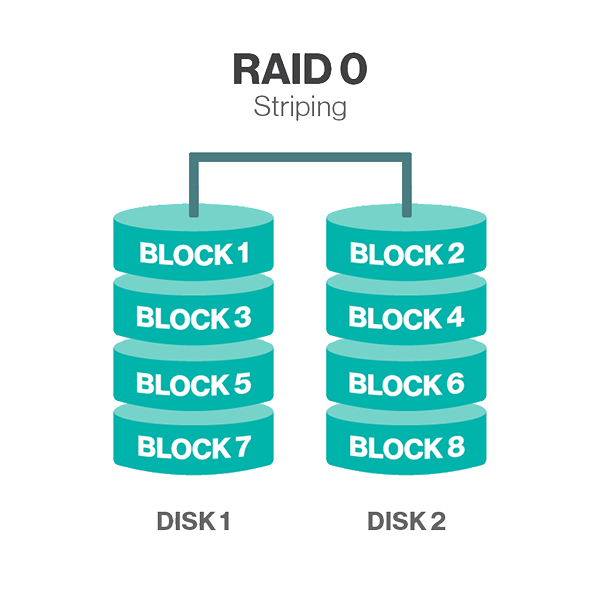
\includegraphics[scale=0.40]{img/raid00.png}
\end{center}
\begin{figure}[htbp]
\caption{Sezionamento senza ridondanza. Questa configurazione ha sezionamento, ma nessuna ridondanza dei dati. Offre migliori prestazioni, ma nessuna tolleranza agli errori \cite{etichetta9}.}
\label{fig:raid00}
\end{figure}

\item 
\verb"RAID 1": livello che si occupa di unire assieme due o pi\`{u} dischi riproducendo fedelmente gli stessi dati. Questa configurazione mantiene quindi almeno una copia esatta di tutti i dati, detta "\textit{mirror}". In questo caso, la rottura di un disco non pregiudica l'utilizzo dei dati che sono disponibili nel disco o nei dischi rimanenti. Pi\`{u} precisamente, l'affidabilit\`{a} aumenta linearmente al numero di dischi presenti: un sistema con \verb"N" dischi \`{e} in grado di resistere alla rottura di \verb"N-1" componenti.\\ La lettura delle prestazioni \`{e} migliorata poich\'{e} entrambi i dischi possono essere letti contemporaneamente. La scrittura delle prestazioni \`{e} la stessa di quella per il singolo disco\cite{etichetta9}. \\
\verb"RAID 1" \`{e} conosciuto anche come \textit{disk mirroring}. Questo tipo di RAID ha la stessa finalit\`{a} della replica.\\


\begin{center}
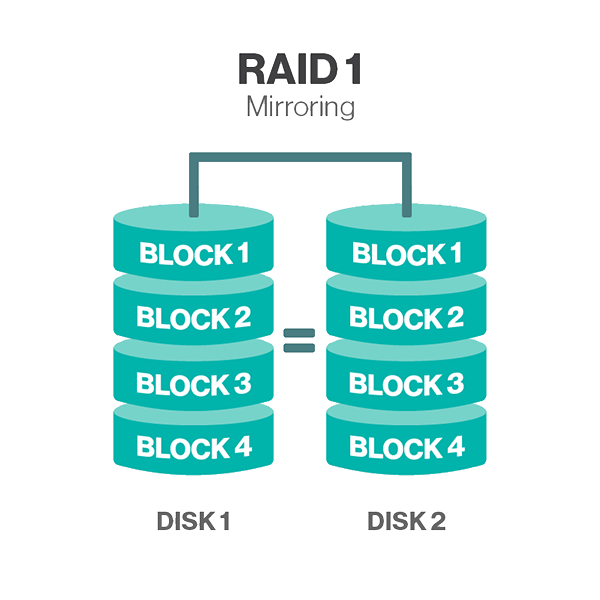
\includegraphics[scale=0.40]{img/raid11.png}
\end{center}

\begin{figure}[htbp]
\caption{Replicazione. Questa configurazione \`{e} costituita da almeno due unit\`{a} che duplicano la memorizzazione dei dati. Non c'\`{e} sezionamento \cite{etichetta9}.}
\label{fig:raid11}
\end{figure}

\item
\verb"RAID 2": livello che divide i dati al livello di bit (invece che di blocco) e usa un \textit{codice di Hamming} per la correzione d'errore che permette di correggere errori su singoli bit e di rilevare errori doppi. Questi dischi sono sincronizzati dal controllore, in modo tale che la testina di ciascun disco sia nella stessa posizione in ogni disco\cite{etichetta10}.\\
%Questa configurazione si rivela molto efficiente in ambienti in cui si verificano numerosi errori di lettura o scrittura, ma in ambienti pi\`{u} prestanti, data l'elevata affidabilit\`{a} dei dischi, il \verb"RAID 2" non viene utilizzato.

\begin{center}
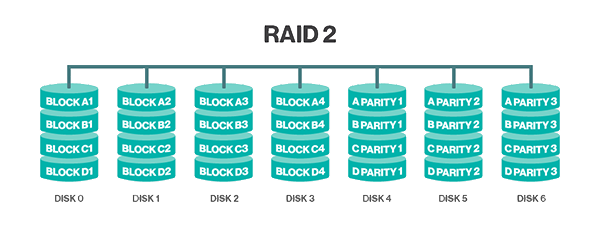
\includegraphics[scale=0.60]{img/raid22.png}
\end{center}
\begin{figure}[htbp]
\caption{Sezionamento a livello di bit. Questa configurazione ha alcuni dischi che memorizzano le informazioni di errore di verifica e correzione (ECC) \cite{etichetta9}.}
\label{fig:raid22}
\end{figure}

\item
\verb"RAID 3": livello che si occupa di unire assieme almeno tre o pi\`{u} dischi, all'interno dei quali i dati vengono suddivisi equamente, in modo da bilanciare anche il carico di operazioni di lettura e scrittura che li riguardano. Dedicano uno di questi dischi al contenimento di un sistema di codici di controllo, che permettono di ricostruire i dati nel caso in cui uno degli altri dischi si rompa. Le informazioni ECC vengono utilizzate per rilevare gli errori. Il recupero dei dati viene effettuato calcolando l'esclusiva \verb"OR" (\verb"XOR") delle informazioni registrate sulle altre unit\`{a} \cite{etichetta9}.\\ 

\begin{center}
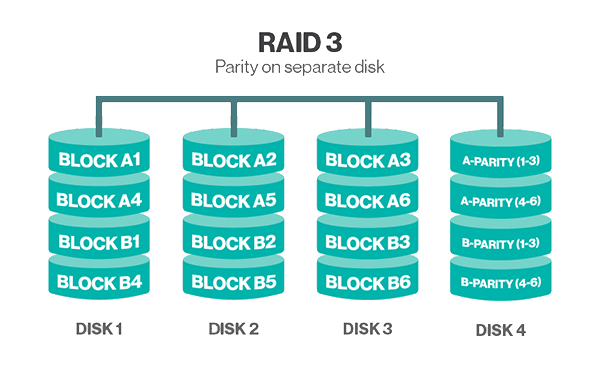
\includegraphics[scale=0.50]{img/raid33.png}
\end{center}
\begin{figure}[htbp]
\caption{Sezionamento a livello di byte con disco di parit\`{a} - Questa configurazione utilizza la rigatura e dedica un'unit\`{a} a memorizzare informazioni di parit\`{a} \cite{etichetta9}.}
\label{fig:raid33}
\end{figure}

\item
\verb"RAID 4": livello simile al livello tre, con la differenza che i dati vengono distribuiti in modo pi\`{u} efficiente tra i dischi, ma rimane compito di un disco separato il sistema di codici di controllo che permette la ricostruzione dei dati, chiamati "blocchi di parit\`{a}".\\
Questo livello utilizza grandi sezionamenti, il che significa che \`{e} possibile leggere i record da un'unica unit\`{a} \cite{etichetta9}.\\

\begin{center}
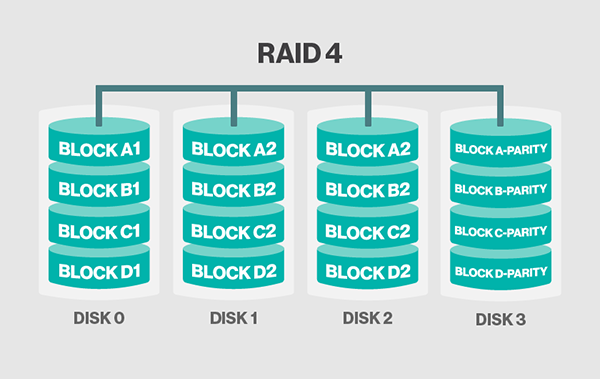
\includegraphics[scale=0.50]{img/raid44.png}
\end{center}

\begin{figure}[htbp]
\caption{Sezionamento a livello di blocco con disco di parit\`{a} \cite{etichetta9}.}
\label{fig:raid44} 
\end{figure}

\item
\verb"RAID 5": livello basato su livello di blocco con parit\`{a} che risiedono su ciascuna unit\`{a}. L'architettura dell'array consente alle operazioni di lettura e scrittura di coprire pi\`{u} unit\`{a}. Ci\`{o} determina prestazioni migliori di quelle di un'unit\`{a} singola, ma non altrettanto elevata di quella di un array \verb"RAID 0" \cite{etichetta9}.\\

\begin{center}
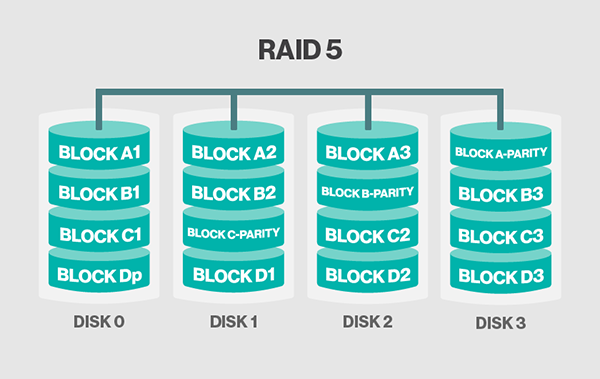
\includegraphics[scale=0.50]{img/raid55.png}
\end{center}

\begin{figure}[htbp]
\caption{Sezionamento a livello di blocco con parit\`{a} distribuita \cite{etichetta9}.}
\label{fig:raid55}
\end{figure}

\item
\verb"RAID 6": livello simile a \verb"RAID 5", ma include un secondo schema di parit\`{a} distribuito attraverso le unit\`{a} nell'array. L'utilizzo di una parit\`{a} aggiuntiva consente all'array di continuare a funzionare anche se due dischi non funzionano contemporaneamente. Tuttavia, questa protezione supplementare \`{e} pi\`{u} costosa. Le matrici RAID \verb"6" hanno un costo superiore a gigabyte (GB) e spesso hanno prestazioni di scrittura pi\`{u} lente degli array \verb"RAID 5"\cite{etichetta9}.\\

\begin{center}
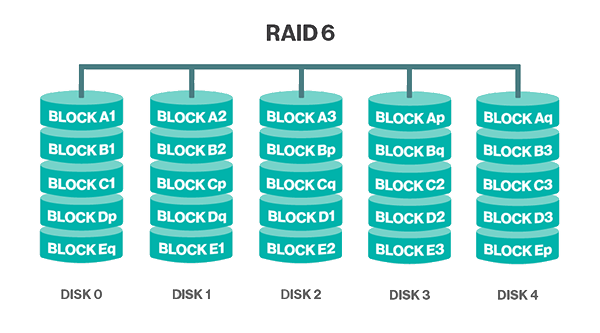
\includegraphics[scale=0.55]{img/raid66.png}
\end{center}

\begin{figure}[htbp]
\caption{Sezionamento a livello di blocco con doppia parit\`{a} distribuita \cite{etichetta9}.}
\label{fig:raid66} 
\end{figure}
\end{itemize}


\paragraph{Livelli RAID nidificati}

I livelli Annidati sono dei tipi di livelli pi\`{u} complessi ottenuti dalla combinazione di alcuni livelli RAID Standard. Esempi classici sono le configurazioni RAID \verb"0+1" o \verb"10".

\begin{itemize}
\item 
\verb"RAID10" (\verb"RAID 1+0"): combinando i \verb"RAID 1" e \verb"0", questo livello viene spesso definito \verb"RAID 10", che offre prestazioni pi\`{u} elevate rispetto al \verb"RAID 1", ma a un costo molto pi\`{u} elevato. In \verb"RAID 1+0", i dati vengono clonati e i \textit{mirror} sono suddivisi in sezioni\cite{etichetta9}.
\end{itemize}

\begin{center}
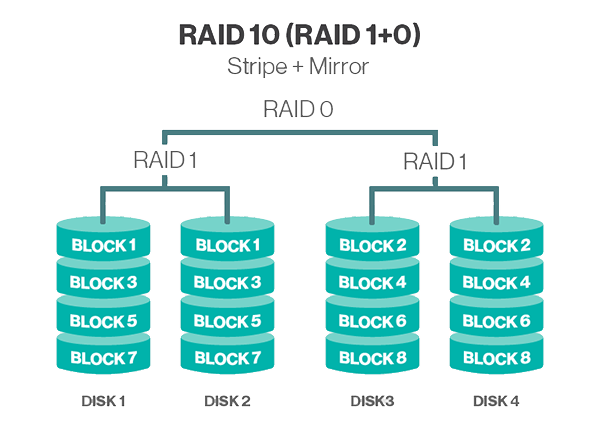
\includegraphics[scale=0.50]{img/raid10.png}
\end{center}

\begin{figure}[htbp]
\caption{Livello RAID nidificato \cite{etichetta9}.}
\label{fig:raid10} 
\end{figure}
\end{itemize}

%%%\textbf{spiegazione cinci -audio-}
%Nelle macchine non distribuite per garantire la ridondanza dei dati si scrive su piu dischi, sincrono (i dati vengono scritti simultaneamente) - come raid mirroring
%%%ci puo essere o un affarino (scheda) chiamato raid controller. Ha una memoria che puoi configurarlo.. puoi dirgli tra disco 1 e disco 2 imponi un raid 0. Quindi che succede? Da una macchina, cioe dal processore, tutte le volte che viene fatta una scrittura su disco, il raid controller la splitta e viene fatta in entrambi i dischi. quindi hai due dischi clonati (mirroring). Stessa cosa del REPLICA.

\item
\subsection{Codice di correzione errore (Erasure Coding)}
La codifica di cancellazione, noto come \emph{Erasure Coding} (EC) \`{e} un metodo di protezione dei dati, i quali vengono suddivisi in frammenti, estesi e codificati con pezzi di dati ridondanti e memorizzati su un insieme di posizioni o supporti di memorizzazione diversi.

L'obiettivo della codifica di cancellazione \`{e} quello di consentire di ricostruire i dati che vengono danneggiati utilizzando le informazioni sui dati memorizzati altrove nell'array. Lo svantaggio della codifica di cancellazione \`{e} che pu\`{o} essere pi\`{u} intenso della CPU e che pu\`{o} tradursi in una maggiore latenza\cite{etichetta11}.

La codifica di cancellazione \`{e} utile con la presenza di grandi quantit\`{a} di dati e tutte le applicazioni o sistemi che devono tollerare i guasti, come sistemi di array a dischi, griglie di dati, applicazioni di archiviazione distribuite. Un caso comune di utilizzo corrente per la codifica di cancellazione \`{e} in un sistema \textit{object-based cloud storage}\cite{etichetta11}.

\subsubsection{Come funziona}
La codifica di cancellazione crea una funzione matematica per descrivere un insieme di numeri in modo che possano essere controllati per l'accuratezza e recuperati in caso di perdita. Questo \`{e} il concetto fondamentale dei metodi di codifica di cancellazione, implementati pi\`{u} frequentemente utilizzando i codici \textit{Reed-Solomon} (tipo di codice lineare (ciclico) non binario di rilevazione e correzione d'errore)\cite{etichetta11}.\\
In termini matematici, la protezione offerta dalla codifica di cancellazione pu\`{o} essere rappresentata in forma semplice dalla seguente equazione:  
\begin{verbatim}
                       		n = k + m
\end{verbatim}
dove:
\begin{itemize}
\item 
la variabile \verb"k" \`{e} la quantit\`{a} originale di dati o simboli; 
\item
la variabile \verb"m" indica i dati aggiuntivi o ridondanti che vengono aggiunti per fornire protezione dai guasti;
\item
la variabile \verb"n" \`{e} il numero totale di dati creati dopo il processo di codifica di cancellazione\cite{etichetta11}.
\item
la variabile \verb"r", chiamata velocit\`{a} di codice, \`{e} definita nel seguente modo: \\
\begin{center}
						\verb"r = "\sqrt{\frac{k}{n}}\\

\end{center}                       		
\end{itemize}
\\
Ad esempio, in una configurazione \verb"10" di \verb"16", o EC \verb"10/16", sei simboli supplementari (\verb"m") saranno aggiunti ai \verb"10" simboli di base (\verb"k"). I \verb"16" frammenti di dati (\verb"n") saranno diffusi su \verb"16" unit\`{a}, nodi o posizioni geografiche. Il file originale potrebbe essere ricostruito da \verb"10" frammenti verificati\cite{etichetta11}.

I codici di cancellazione, noti anche come codici di correzione degli errori di avanzamento (FEC), sono stati sviluppati pi\`{u} di \verb"50" anni fa. Da quel momento sono emersi diversi tipi. In uno dei tipi pi\`{u} comuni, \textit{Reed-Solomon}, i dati possono essere ricostruiti utilizzando qualsiasi combinazione di simboli \verb"k" o pezzi di dati, anche se i simboli \verb"m" sono persi o non sono disponibili. Ad esempio, in EC \verb"10/16", sei unit\`{a}, nodi o posizioni geografiche potrebbero essere persi o non disponibili e il file originale sar\`{a} ancora recuperabile\cite{etichetta11}.
 
\item
\section{Software utilizzato per gli esperimenti}
\item
\subsection{PosgreSQL}
PostgreSQL \`{e} un potente sistema \textit{open source} di database relazionale (DBMS, \textit{Database Management System}) cio\`{e} \`{e} un sistema software progettato per consentire la creazione e manipolazione efficiente di database, ovvero di collezioni di dati strutturati.\\ 
Ha pi\`{u} di \verb"15" anni di sviluppo attivo e un'architettura collaudata che ha guadagnato una notevole reputazione per l'affidabilit\`{a}, l'integrit\`{a} e la salvaguardia dei dati allocati e la correttezza di archiviazione.

PostgreSQL \`{e} un sistema di gestione dei database relazionale (\textit{Object-Relational}, acronimo ORDBMS) basato su Postgres, sviluppato presso l'Universit\`{a} della California presso il Dipartimento di Informatica di Berkeley\cite{etichetta15}.\\
Funziona su tutti i principali sistemi operativi, tra cui Linux, UNIX (AIX, BSD, HP-UX, SGI IRIX, Mac OS X, Solaris, Tru\verb"64"), e Windows\cite{etichetta15}.\\

Supporta gran parte dello standard SQL e offre molte funzionalit\`{a} moderne:
\begin{itemize}
\item 
\textit{queries} complesse;
\item
foreign keys;
\item
triggers;
\item
views aggiornabili;
\item
integrit\`{a} transazionale;
\item
controllo della concorrenza multiversione.
\end{itemize}

%Permette di aggiungere funzioni personalizzate sviluppate utilizzando diversi linguaggi di programmazione quali C/C++, Java, Perl, Python, Ruby, Tcl e Open Database Connectivity (ODBC).

Seguono le caratteristiche principali di PostgreSQL; le funzionalit\`{a} introdotte nella recente versione \verb"9.1" :
\begin{itemize}
\item 
elevata aderenza agli standard SQL;
\item 
architettura\textit{ client-server} con una gamma completa di driver e di client;
\item 
progettato in modo altamente concorrente, evitando che i processi in scrittura blocchino i processi in lettura;
\item 
altamente configurabile ed estendibile, consentendo svariati tipi di applicazioni;
\item 
elevate scalabilit\`{a} e prestazioni, unite a un ampio spettro di possibilit\`{a} per tarare la configurazione;
\item 
sofisticato ottimizzatore delle query;
\item 
supporto completo per Java, Python, Perl, PHP e molti altri linguaggi, sia per le procedure interne al server di database che per l'accesso da parte di client;
\item 
elevata affidabilit\`{a}, con una vasta serie di caratteristiche per durabilit\`{a} e alta disponibilit\`{a}\cite{etichetta12}.
\end{itemize}\\

PostgreSQL \`{e} progettato per essere estensibile, poich\'{e} \`{e} possibile definire i propri tipi di dati, tipi di indici e lingue funzionali. Offre un ricco set di strumenti per gli sviluppatori in modo da gestire l'accesso simultaneo ai dati. Inoltre vi \`{e} la possibilit\`{a} di ottimizzarlo per soddisfare le proprie esigenze, tramite uno sviluppo di un plugin personalizzato.

Un database di classe enterprise, PostgreSQL vanta funzionalit\`{a} sofisticate come il controllo della concorrenza multiversione, il ripristino in tempo reale (\textit{point in time recovery}), \textit{tablespaces}, replica asincrona, transazioni nidificate (\textit{savepoints}), backup in linea/a caldo, un sofisticato query planner/optimizer, ed il \textit{write ahead logging} per una maggiore tolleranza ai guasti.\\
\`{E} estremamente scalabile sia nella quantit\`{a} pura di dati che pu\`{o} gestire sia nel numero di utenti concorrenti che pu\`{o} ospitare\cite{etichetta15}.\\

Alcuni limiti generali di PostgreSQL sono inclusi nei punti riportati di seguito:\\

\begin{tabular}{|l|l|r|}
%seconde parantesi 1cr se non vuoi linee e togli \hline
\hline
Dimensione massima del database & Illimitato\\
\hline
Dimensione massima Tabella & \verb"32 TB"\\
\hline
Dimensione massima Riga & \verb"1,6 TB"\\
\hline
Dimensione Massima campo & \verb"1 GB"\\
\hline
Numero Massimo Righe per tabella & Illimitato\\
\hline
Numero Massimo colonne per la tabella & \verb"250 - 1600"\\
%a seconda dei tipi di dati delle colonne\\
\hline
Numero Massimo indici per la tabella & Illimitato\cite{etichetta12}\\
\hline
\end{tabular}\\

\subsubsection{Controllo concorrenza multiversione (MVCC)}
MVCC (\textit{Multi-Version Concurrency Control}) \`{e} una tecnica avanzata per migliorare le prestazioni del database in un ambiente multiutente, mantenendo la coerenza dei dati. \\
A differenza della maggior parte degli altri sistemi di database che utilizzano i \textit{lock} per il controllo della concorrenza, Postgres mantiene la coerenza dei dati utilizzando questo modello. \\
Ci\`{o} significa che durante l'interrogazione di un database ogni transazione vede un'istantanea di dati (una versione del database), indipendentemente dallo stato corrente dei dati sottostanti. Questo protegge la transazione dalla visualizzazione di dati incoerenti che potrebbero essere causati da altri eventuali aggiornamenti simultanei delle transazioni sulle stesse righe di dati, fornendo l'isolamento della transazione per ciascuna sessione del database\cite{etichetta15}.\\

La differenza principale tra i modelli multiversione e di blocco \`{e} che nei blocchi MVCC acquisiti per la query (lettura) i dati non sono in conflitto con i blocchi acquisiti per la scrittura dei dati e quindi la lettura non blocca mai la scrittura e la scrittura non blocca mai la lettura.

\subsubsection{Caratteristiche PostgreSQL}
Mentre PostgreSQL ha un catalogo di sistema completamente relazionale che supporta pi\`{u} schemi per database, il suo catalogo \`{e} accessibile anche attraverso lo schema di informazioni definito nello standard SQL.

Le funzionalit\`{a} di integrit\`{a} dei dati includono le chiavi primarie (combinate), le chiavi estranee con aggiornamenti e cancellazioni a cascata, i controlli dei vincoli, i vincoli unici e non i vincoli nullo.

Ha anche una serie di estensioni e funzionalit\`{a} avanzate. PostgreSQL supporta indici composti, unici, parziali e funzionali che possono utilizzare qualsiasi metodo di archiviazione \textit{B-tree}, \textit{R-tree}, \textit{hash} o GiST\cite{etichetta15}.\\

Altre funzionalit\`{a} avanzate includono l'ereditariet\`{a} delle tabelle, i sistemi di regole e gli eventi del database. L'ereditariet\`{a} di tabelle mette un orientamento orientato all'oggetto sulla creazione della tabella, consentendo ai progettisti di database di derivare nuove tabelle da altre tabelle, trattandole come classi di base.\\
Di fatto, PostgreSQL supporta sia l'ereditariet\`{a} singola che quella multipla.\\

Il sistema di regole, chiamato anche il sistema di riscrittura delle query, consente al progettista di creare regole che identificano operazioni specifiche per una determinata tabella o vista e le trasformano dinamicamente in operazioni alternative quando vengono elaborate.\\
Il sistema eventi \`{e} un sistema di comunicazione interprocesso in cui i messaggi e gli eventi possono essere trasmessi tra i client utilizzando i comandi \verb"LISTEN" e \verb"NOTIFY", consentendo sia la semplice comunicazione \textit{peer-to-peer} sia un coordinamento avanzato sugli eventi del database. Poich\'{e} le notifiche possono essere rilasciate da \textit{trigger} e procedure salvate, i client PostgreSQL possono monitorare eventi di database come gli aggiornamenti, gli \verb"insert" o le eliminazioni di tabella quando vengono eseguiti\cite{etichetta15}.

\subsubsection{Elevata personalizzazione}
PostgreSQL esegue procedure memorizzate in pi\`{u} di una dozzina di linguaggi di programmazione, tra cui Java, Perl, Python, Ruby, Tcl, C/C++ e il proprio PL/pgSQL, simile a PL/SQL di Oracle. \\
I \textit{trigger} e le procedure salvate possono essere scritti in C e caricati nel database come libreria, permettendo una grande flessibilit\`{a} nell'estensione delle sue funzionalit\`{a}. Allo stesso modo, PostgreSQL include un \textit{framework} che consente agli sviluppatori di definire e creare i propri tipi di dati personalizzati insieme a funzioni di supporto e operatori che definiscono il loro comportamento.\\

Il codice sorgente di PostgreSQL \`{e} disponibile sotto una licenza libera open source: la licenza PostgreSQL. Questa licenza d\`{a} la libert\`{a} di utilizzare, modificare e distribuire PostgreSQL in qualsiasi forma, sorgente aperta o chiusa\cite{etichetta15}.\\

Non esiste un unico formato per tutti i software di replica. \`{E} necessario capire le proprie esigenze e come si adattino diversi approcci.\\
%\textbf{(spiegazione cinci -audio-)}
%Uno dei punti di forza che ha reso famoso e versatile Posgres è che è un (Database Management System è un sistema software progettato per consentire la creazione e manipolazione efficiente di database (ovvero di collezioni di dati strutturati) ) (scritto in C). Ha dei rametti dove te riesci ad agganciarci dei software fatti ad OC. te ti agganci a un sistema di segnalistica interna e lui quindi tramite messaggi di scambio interno ti permette di lavorare (ti dice "ho fatto l'inserimento di questa tabella(INSERT), ti scatta il segnale, e te riesci a intercettare e quindi fare delle operazioni)

%Pg Logical è un estensione di Posgres. Lui capisce quando fa inserimenti e riesce a duplicare soltando parti di database. Mentre replica di posgres per adesso ti replicherebbe tutto il DB. Invece noi si fa con solo tabelle (R) o quanti record di tabelle (per id maggiori di x) adirittura si vogliono replicare o colonne di tabelle \\
La replica delle modifiche dello schema \`{e} un problema frequentemente discusso e solo pochi sistemi di database forniscono le estensioni necessarie per implementarlo. PostgreSQL non fornisce la possibilit\`{a} di definire i trigger richiamati sulle modifiche dello schema, quindi un modo trasparente per replicare le modifiche dello schema non \`{e} possibile senza un sostanziale lavoro nel sistema centrale di PostgreSQL.\\
Il sistema di replica Pglogical avr\`{a} un meccanismo per eseguire script SQL in modo controllato come parte del processo di replica.

\item
\subsubsection{Write-Ahead Loggin (WAL)}
\textit{Write-Ahead Logging} (WAL) \`{e} un metodo standard per garantire l'integrit\`{a} dei dati. Il concetto centrale di WAL \`{e} che le modifiche ai file di dati (dove risiedono tabelle e indici) devono essere scritte solo dopo che tali modifiche sono state registrate, ovvero dopo che i record di registro che descrivono le modifiche sono stati scaricati nella memoria permanente. Se viene seguita questa procedura, non abbiamo bisogno di svuotare le pagine di dati sul disco su ogni \verb"commit" di transazione, perch\'{e} sappiamo che in caso di \textit{crash} saremo in grado di recuperare il database usando il log: eventuali modifiche che non sono state applicate alle pagine di dati possono essere rifatte dai record del registro. Questo \`{e} il recupero \textit{roll-forward}, noto anche come REDO.\\

Poich\'{e} WAL ripristina il contenuto del file di database dopo un arresto anomalo, i \textit{filesystem} registrati non sono necessari per l'archiviazione affidabile dei file di dati o dei file WAL. \\
%In effetti, l'overhead del journaling può ridurre le prestazioni, specialmente se l'inserimento nel journal fa sì che i dati del file system vengano scaricati su disco. Fortunatamente, lo svuotamento dei dati durante l'inserimento nel journal può spesso essere disabilitato con un'opzione di montaggio del file system, ad es. data = writeback su un file system Linux ext3. I file system journalizzati migliorano la velocità di avvio dopo un arresto anomalo.
L'utilizzo di WAL determina un numero notevolmente ridotto di scritture su disco, poich\'{e} \`{e} necessario scaricare il file di registro sul disco per garantire che una transazione venga eseguita, piuttosto che ogni file di dati modificato dalla transazione. \\
Il file di registro viene scritto in modo sequenziale e pertanto il costo della sincronizzazione del log \`{e} molto inferiore al costo dello svuotamento delle pagine di dati. Ci\`{o} \`{e} particolarmente vero per i server che gestiscono molte piccole transazioni toccando diverse parti dell'archivio dati\cite{etichetta15}.
 
\item
\subsection{Pglogical}
Pglogical \`{e} un sistema logico di replica implementato come estensione di PostgreSQL. Completamente integrato, non richiede alcun triggers o programmi esterni. Questa alternativa alla replica fisica \`{e} un metodo altamente efficiente per replicare i dati utilizzando un modello di \textit{publish/subscriber} per la replica selettiva\cite{etichetta3}.
%Metodo di replicazione : Master-Slave

\subsubsection{Vantaggi}
I vantaggi offerti da Pglogical sono i seguenti:
\begin{itemize}
\item
replica sincrona;
\item
replica ritardata;
\item
risoluzione dei conflitti configurabili;
\item
capacit\`{a} di convertire lo \textit{standby} fisico in una replica logica;
\item
le sequenze possono essere replicate;
\item
nessun \textit{trigger}; questo significa ridurre il carico di scrittura sul \textit{Provider};
\item
nessuna re-esecuzione di SQL significa overhead e latenza ridotti per il sottoscrittore;
\item
non \`{e} necessario annullare le query per consentire alla replica di continuare la riproduzione;
\item
il sottoscrittore (\textit{subscriber}) pu\`{o} avere diversi utenti e protezione, indici diversi, impostazioni di parametri diversi;
\item
replica solo un database o un sottoinsieme di tabelle, noto come set di replica (\textit{Replication Sets});
\item
replica in versioni o architetture di PostgreSQL, consentendo aggiornamenti a bassa o \textit{zero-downtime};
\item
pi\`{u} server a monte in un singolo \textit{subscriber} per l'accumulo di cambiamenti\cite{etichetta3}.
\end{itemize}

\subsubsection{Casi di uso}
I diagrammi che seguono descrivono i gestori di database delle funzioni che sono eseguibili con Pglogical:

Migrare e aggiornare PostgreSQL con tempi di inattivit\`{a} quasi a zero: 

\begin{center}
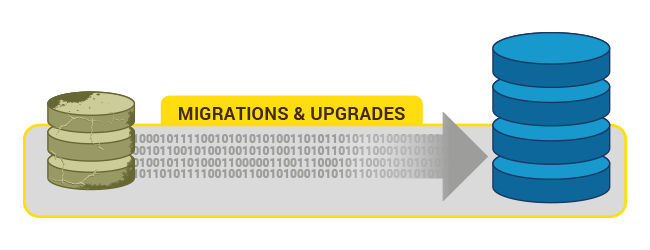
\includegraphics[scale=0.60]{img/pglogical_1.png}\\
\end{center}
\begin{figure}[htbp]
\caption{Migrazione e aggiornamenti PostgreSQL \cite{etichetta3}.}
\label{fig:pglogical_1}
\end{figure}

Accumulare le modifiche provenienti da server di database scartati in un data \textit{warehouse}:

\begin{center}
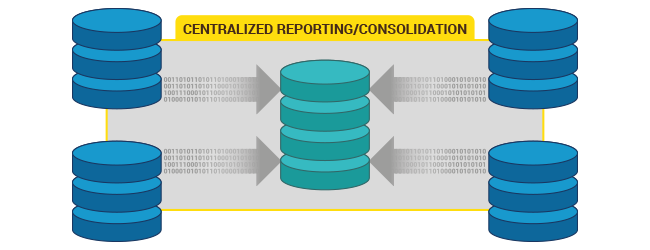
\includegraphics[scale=0.60]{img/pglogical_2.png}\\
\end{center}
\begin{figure}[htbp]
\caption{Aggregazione \cite{etichetta3}.}
\label{fig:pglogical_2}
\end{figure}

Copiare tutti o una selezione di tabelle di database ad altri nodi di un cluster:

\begin{center}
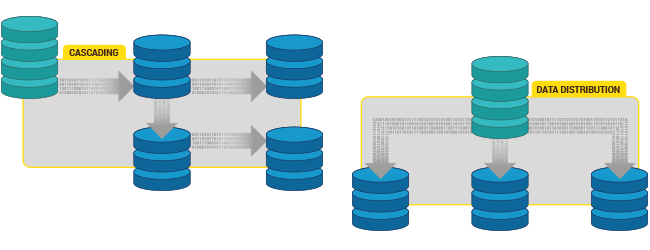
\includegraphics[scale=0.60]{img/pglogical_3.png}\\
\end{center}
\begin{figure}[htbp]
\caption{A cascata e distribuzione dati \cite{etichetta3}.}
\label{fig:pglogical_3}
\end{figure}

Le modifiche del database in tempo reale ad altri sistemi:

\begin{center}
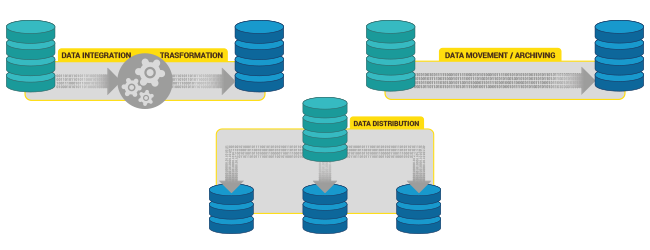
\includegraphics[scale=0.60]{img/pglogical_4.png}\\
\end{center}
\begin{figure}[htbp]
\caption{A cascata e distribuzione dati \cite{etichetta3}.}
\label{fig:pglogical_4}
\end{figure}


\subsubsection{Come funziona pglogical?}
Pglogical utilizza le funzioni di decodifica logica aggiunte da 2ndQuadrant (e disponibili da PostgreSQL \verb"9.4"). \\
Pglogical funziona ancora pi\`{u} veloce con PostgreSQL \verb"9.5" e successive, con bassi \textit{overhead} su entrambi i \textit{provider} e i \textit{subscribers}.\\
Pglogical si basa molto sulle caratteristiche introdotte nell'ambito dello sviluppo BDR (\textit{Bi-directional replication}), tra cui:

\begin{itemize}
\item
decodifica logica;
\item
slot di replica;
\item
origini di replica;
\item
impegnano \verb"timestamp";
\item
messaggi WAL logici\cite{etichetta3}.
\end{itemize}

Pglogical non fornisce funzionalit\`{a} complete di replica \textit{multi-master} e un supporto di modifica dello schema coerente, come fa la BDR. Pglogical incorpora le funzionalit\`{a} di BDR per produrre una soluzione pi\`{u} semplice da utilizzare per la replica unidirezionale, utilizzabile da pi\`{u} utenti per una vasta gamma di casi di utilizzo. \\
Lo sviluppo di BDR \`{e} utilizzato per scenari che richiedono piena capacit\`{a} \textit{multi-master}, riutilizzando gran parte del codice da Pglogical\cite{etichetta3}.\\

Utilizziamo i seguenti termini per descrivere i flussi di dati tra host:

\begin{itemize}
\item
Nodi: istanze del database PostgreSQL
\item 
\textit{Provider/Subscibers}: ruoli presi dai nodi
\item 
\textit{Replication set} o set di replica: una raccolta di tabelle che identificano i dati da replicare.
\end{itemize}

I casi d'uso supportati sono:
\begin{itemize}
\item 
replica completa del database;
\item 
replica selettiva di insiemi di tabelle mediante set di repliche;
\item 
replica selettiva delle righe della tabella sul lato del \textit{publisher} o del sottoscrittore (\verb"row_filter");
\item 
replica selettiva delle colonne della tabella sul lato del \textit{master}\cite{etichetta3}.
\end{itemize}

\item
\section{Hardware utilizzato per gli esperimenti}
Il lavoro presentato in questa tesi analizza l'esecuzione di test su un determinato tipo di hardware.\\

Le reti sono orientate in due LAN per avere alta disponibilit\`{a} del dato (\textit{high-ability}). \`{E} possibile contattare lo stesso microserver su due differenti porte Ethernet.\\
Una semi-unit\`{a} che supporta fino a \verb"6" microserver e \verb"6" hard disk. Ha alimentazione dedicata a gruppi di \verb"6" e ventole di raffreddamento.

\begin{center}
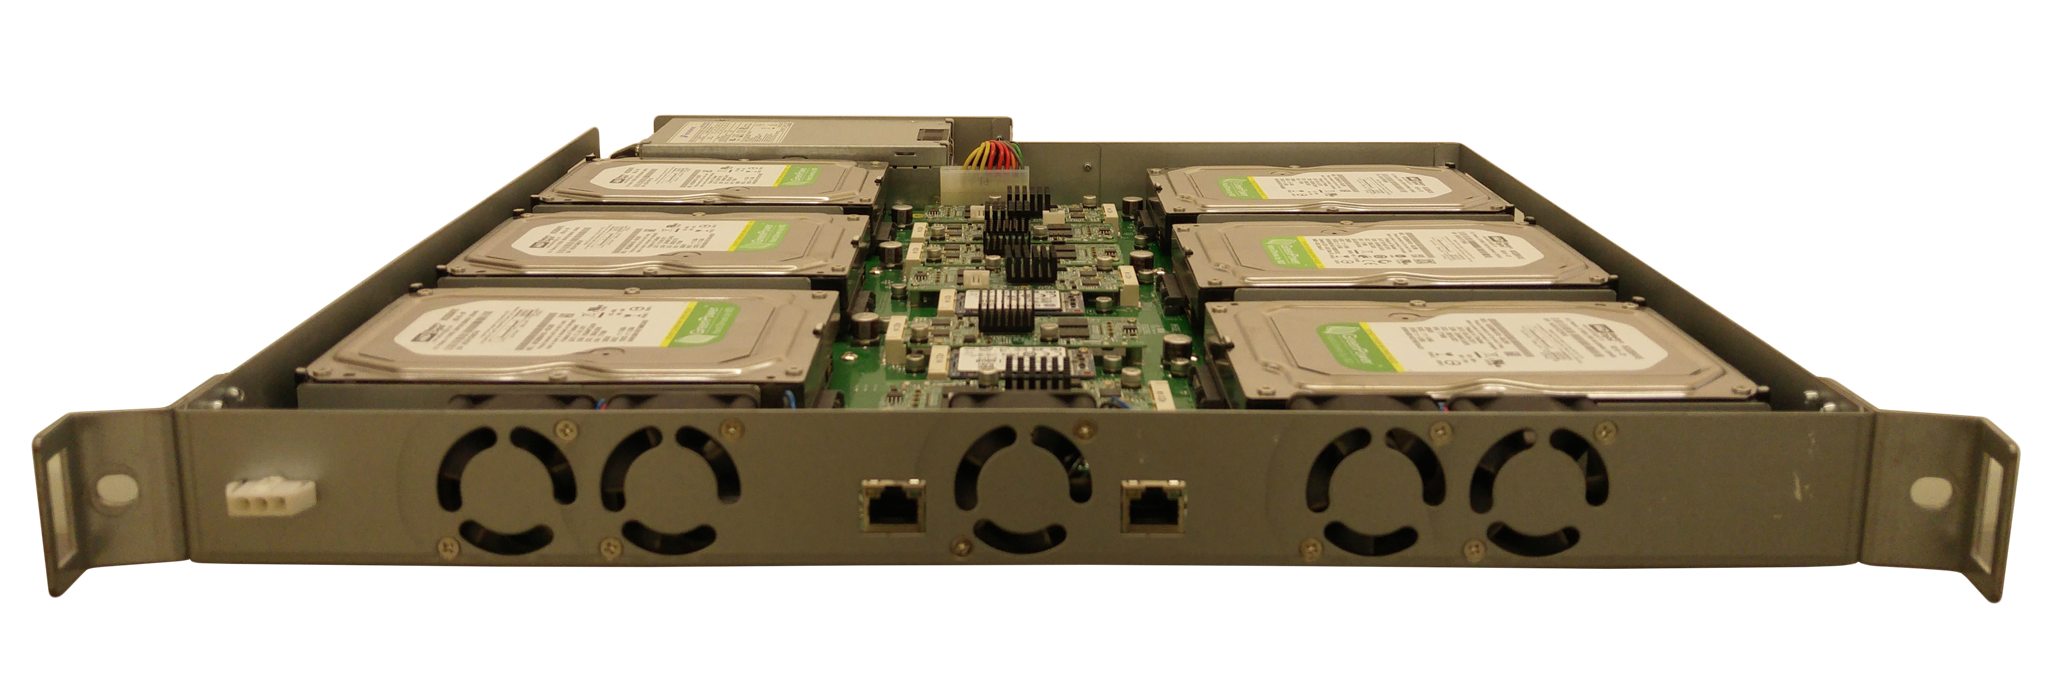
\includegraphics[scale=0.20]{img/CY7.png}\\
\end{center}
\begin{figure}[htbp]
\caption{Sei microserver e sei hard disk. \label{fig:CY7}}
\end{figure}

Ci sono due semi-unit\`{a} per ogni piano \textit{rack}, inserite come illustrato dalla seguente figura:

\begin{center}
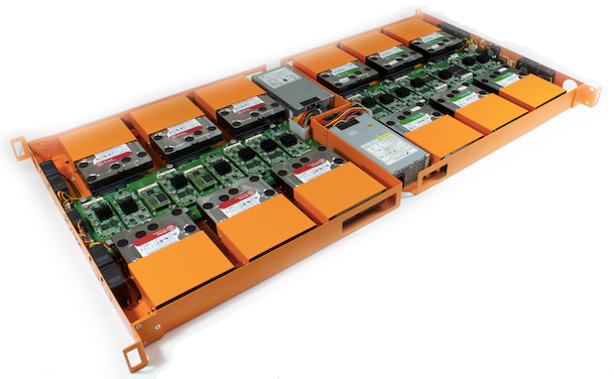
\includegraphics[scale=0.40]{img/CY7x2.png}
\end{center}
\begin{figure}[htbp]
\caption{Due semi-unit\`{a}. \label{fig:CY7x2}}
\end{figure}

Segue un illustrazione di un \textit{rack}. Alla sommit\`{a} ci sono due \textit{switch} di rete:

\begin{center}
\begin{figure}[htbp]
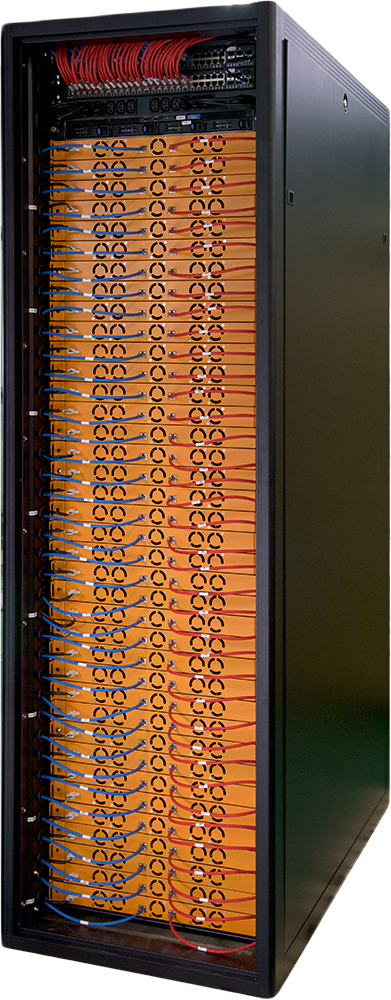
\includegraphics[scale=0.30]{img/rack.png}
\caption{Un rack. \label{fig:rack}}
\end{figure}
\end{center}
